\scanpage{16}
% archive foliation: 15
Soit $G$ un groupe, $C_G$ la catégorie des ensembles $E$ où $G$ opère \inserted{à \deleted{droite} gauche}, et tels que $E/G$ soit fini. On sait que la catégorie des hyperfaisceaux d'ensembles sur $C_G$ (\deleted{pour} les épimorphismes dans $C_G$ comme morphismes de descente) est équivalente à la catégorie des ensembles \deleted{(quelconques)} où $G$ opère à \deleted{droite} \inserted{gauche} ; si $A$ est un tel, $\Phi_A$ l'hyperfaisceau associé, on a
\margin{à développer}\figure{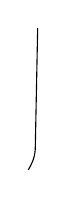
\begin{tikzpicture}\draw (0,0)--(-0.03,-1.5) to[out=-90,in=60] (-0.12,-1.8);\end{tikzpicture}}
\[
\Phi_A(\deleted{\unsure{E}}X)=\deleted{A\times_{(G)}\unsure{X}\times_{(G)}A}\operatorname{Hom}_G(X,E)
\]
\deleted{Ainsi, \unsure{étant donné}, la \unsure{donnée}\unsure{?}}

Et si $\Phi$ est un hyperfaisceau, alors l'ensemble à opérateurs associé est
\[
A=\Phi(G_g)
\]
où $G_g$ désigne $G$ considéré comme ens. à groupe d'opérateurs à gauche $G$ par l'op. rég. gauche.

\deleted{Soit $F$ un sous-groupe de $G$, et soit $C_{G;F}$ la sous-catégorie de $C_G$ formée des $X\in C_G$ tels que $F$ y opère \unsure{trivialt} ; c'est une sous-catégorie stable pour les opérations habituelles [sommes, \unsure{lim}, produits fibrés, quotients et \unsure{foncteurs} $\operatorname{Hom}$].}
